\documentclass[margin]{res}
\usepackage[icelandic]{babel}
\usepackage[T1]{fontenc}
\usepackage[utf8x]{inputenc}
\usepackage{graphicx}
\usepackage{url}
\setlength{\textwidth}{5.1in}

\begin{document}
\begin{figure}
\begin{minipage}[b]{0.45\linewidth}
\section {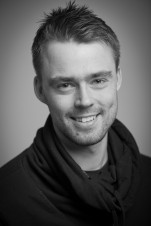
\includegraphics[height=4.8cm]{hlysig_profile}}
\end{minipage}
\hspace{0.5cm}
\begin{minipage}[b]{0.45\linewidth}
{\large\bf Hlynur Sigurþórsson}\\
 Seilugrandi 9\\
 107, Reykjavík Iceland\\
 hlysig@gmail.com\\
 Mobile: (+354) 893-1000\\
\end{minipage}
\end{figure}

\begin{resume} 
\section{PERSONAL DETAILS}
Born January 10, 1985, Reykjavík Iceland. Icelandic Citizenship. Married to
Thelma Björk Wilson (Icelandic and Canadian Citizenship) who is currently
completing her masters degree in Engineering Management this summer and works
as a flight attendant at IcelandAir\footnote{\url{http://www.icelandair.com/}}.
We currently live in Reykjavík, Iceland.

\section{OBJECTIVE}  
A position in the field of computers with interests in application development,
large scale application architectures, distributed systems and web technology
in general. Currently I obtain a position as a senior developer at
Azazo\footnote{\url{http://www.azazo.com}} where we develop a cloud based
document storage for customers. I also hold a position as a part time teacher
at the Reykjavík University\footnote{\url{http://www.ru.is}}.

\section{EDUCATION}
2011: \emph{M.Sc.,} Computer Science, Reykjavík University, thesis title is
\emph{PhotoCube: A Multi-Dimensional Image Browser}

2009: \emph{B.Sc.,}
Computer Science, Reykjavík University, report title is \emph{Using IceNLP in
Computer-Assisted Language Learning.} 

\section{TEACHING}
2014 - Spring:\\
Computer Science Final Project (T-404-LOKA), Supervisor and moderator over 4
projects at Reykjavík University.

2013 - Fall:\\ 
Computer Graphics (T-511-TGRA), Teacher assistant at Reykjavík University.
Computer Science Final Project (T-404-LOKA), Supervisor and moderator over 4
projects at Reykjavík University.

2013 - Spring:\\ 
Computer Science Final Project (T-404-LOKA), Supervisor and moderator over 4
projects at Reykjavík University. Web Programming (T-213-VEFF), Teacher at
Reykjavík University.

2012 - Fall:\\ 
Computer Graphics (T-511-TGRA), Teacher assistant at Reykjavík University.
Computer Science Final Project (T-404-LOKA), Supervisor and moderator over 4
projects at Reykjavík University.

2012 - Spring:\\ 
Supervisor over undergraduate final projects at Reykjavík University, Assistant Supervisor in M.Sc., thesis title is \emph{A Face Recognition Plug-in for the PhotoCube Browser.} at Reykjavík University. Computer Science Final Project (T-404-LOKA), Supervisor and moderator over 4 projects at Reykjavík University.

2011 - Spring:\\ 
Computer Science Final Project (T-404-LOKA), Supervisor and moderator over 4 projects at Reykjavík.

\section{PUBLICATIONS}
Björn Þór Jónsson, Áslaug Eiríksdóttir, Ólafur Waage, Grímur Tómasson, Hlynur Sigurþórsson, Laurent Amsaleg. 
M3 + P3 + O3 = Multi-D Photo Browsing. 
In 20th Anniversary International Conference on MultiMedia Modeling (MMM), Dublin, Ireland, January, 2014.

Grímur Tómasson, Hlynur Sigurþórsson, Kristján Rúnarsson, Gísli Kristján Ólafsson, Björn Þór Jónsson, Laurent Amsaleg. 
Using PhotoCube as an Extensible Demonstration Platform for Advanced Image Analysis Techniques (demonstration paper). 
In Tenth International Workshop on Content-Based Multimedia Indexing (CBMI), Annecy, France, June, 2012.

Grímur Tómasson, Hlynur Sigurþórsson, Björn Þór Jónsson, Laurent Amsaleg. 
PhotoCube: Effective and Efficient Multi-Dimensional Browsing of Personal Photo Collections (demonstration paper). 
In ACM International Conference on Multimedia Retrieval (ICMR), Trento, Italy, April, 2011.

Martha Dís Brandt, Hrafn Loftsson, Hlynur Sigurþórsson and Francis M. Tyers. 2011. Apertium-IceNLP: A rule-based Icelandic to English machine translation system. In Proceedings of the 15th Annual Conference of the European Association for Machine Translation (EAMT-2011). Leuven, Belgium.


\section{GUEST LECTURES}

2013: \emph{GIT Version control}. Guest speaker in the course T-303-HUGB Software engineering at Reykjavík University.

2012: \emph{The power of the shell}. Guest lecturer for the course Scripting and Linux Admin (T-426-SCLI). Topic: Interactive session in configuring web servers using Apache, MySQL, PostgreSQL, Python and PHP.

2012: \emph{The power of the shell}. Guest lecturer for the course Software Engineering. Topic: Interactive tutorial in a Linux shell and GIT. 

 

\section{EXPERIENCE}
{\sl Senior developer at Azazo} \hfill 2012 - Present \\
Gagnavarslan is an innovative company that has developed CoreData ECM, a suite of software service that help customers manage their electronic information, documents and records. 
I am currently part of the core developer team which is responsible for the whole application stack and the architectural design of the software.

Contact information:
\begin{itemize}\itemsep -3pt
\item Bæjarhraun 22, 220 Hafnarfirði, Iceland
\item http://www.azazo.com
\item (+354) 553-1000
\end{itemize}

Supervisors:
\begin{itemize} \itemsep -3pt
 \item Jónas Sigurðsson (jonas@azazo.com)
 \item Hannes Pétursson (hannes@azazo.com)
\end{itemize}

{\sl Research developer} \hfill 2011 \\
Working with Dr. Hrafn Loftsson on Daemonizing and enhancing IceNLP. The goal
of the project was to modify the IceNLP toolkit to integrate it into the
Apertium platform.  Project report title is \emph{Daemonizing and enhancing
IceNLP for the purpose of machine translation.}\\ Supervisor Dr. Hrafn Loftsson
(hrafn@ru.is).

{\sl Applications developer at Samskip Holding B.V.} \hfill 2009 - 2012 \\
Samskip is one of the larger container transport companies in Europe with over
1000 employees. I was part of the IT Systems Development team which write
indoor software for their operation. My responsibilities were mostly within 

\begin{itemize}
\item Business intelligence
\item Integration solutions
\item Web applications
\end{itemize}

My supervisor at Samskip was Vignir Jónsson (vignir.jonsson@samskip.com).

{\sl Applications developer at Landsbanki Íslands} \hfill Summer 2008 \\
Landsbankinn is a leading Icelandic financial institution. I was part of the
CRM team where the main focus was to integrate Microsoft WorkFlow Foundation
into their client Architecture.  My supervisor at Landsbankinn was Björgvin
Áskelsson.

{\sl Service Desk operator at Samskip} \hfill Summer 2007 \\
My supervisor at Samskip was Ægir Pálsson (aegir.palsson@samskip.com).


\section{SKILLS} 
{\sl Programming Languages}: Programming languages that I use in my projects
are C$++$, C\#, Java, Python, Ruby, HTML, CSS, JavaScript and SQL. I have no
problems adopting to new languages especially if they fall under the category
of Object-orient programming languages. I am also interested in functional
programming languages and I have been experimenting with both Haskell and
Erlang.

{\sl Software development:}
I consider myself to have a deep understanding of operating systems and
development and the ability to combine this knowledge in order to create
enterprise applications. I have been part of writing a number of large scale
distributed systems.

{\sl Operating Systems:} Windows, Windows server, Unix-like operating systems.
I use Linux and OS X as primary operating systems.

{\sl Languages:} I speak both Icelandic and English fluently.

{\sl Personal:}
I am a team player with excellent communication skills, reliable, flexible and
hard working. I have mostly worked on self-organizing independent teams and I
thrive on sharing and learning from other developers. I am passionate about
designing and developing applications and seeing them grow.

\section{GRANTS}
The PhotoCube Image Browser
(Student Innovation Fund Grant) with Grímur Tómasson and Björn Þór Jónsson.

\section{HONORS}
Reykjavík University, Dean’s List of Distinguished Students.\\
The local Citizenship winner and Idea Cup 1st price winner, Microsoft Imagine
Cup, Optimizing Expenditure on cycling roads using the GPS data collected by
cyclists.

\section{ACTIVITIES \& HOBBIES}
Computers and the field of computer science occupy large chunk of my "hobbies
cake". I spend an enormous amount of time reading books, blog entries and open
source projects.

I believe that physical exercising is a prerequisite for productivity.
Therefore I train Olympic weightlifting. I am interested in environmentally
friendly transportation and I travel mostly by cycling.

I am a big fan of Sci-fi movies and in my free time play the guitar and try out
new exotic beers. Most of all, I love travelling with my wife and walk around
new streets.
\end{resume}
\end{document}
